\documentclass{beamer}
\usepackage{remreset}
\usepackage{etoolbox}
\usepackage{comment}
\usepackage{graphicx}
%\usepackage{dtklogos}
\usepackage{dsfont}
\usepackage{amsmath,amssymb}
\usepackage{tikz} 
\usepackage{cancel}
\setbeamercovered{invisible}


\makeatletter
\@removefromreset{subsection}{section}
\patchcmd{\beamer@part}{\setcounter{subsection}{0}}{}{}
\makeatother
\setcounter{subsection}{1}
\setbeamercovered{transparent}

\mode<presentation>{}
%% preamble
\title[Income Uncertainty and Consumption Dynamics]{Income Uncertainty and Consumption Dynamics}
\author{Edmund Crawley \& Andreas Kuchler}
%\date[2/27/2018]{February 27, 2018}
\usetheme{Frankfurt}
\begin{document}


\frame{\titlepage}

\section{Motivation}
\setbeamercovered{invisible}
\frame
{
	\frametitle{Overview}
	1) How well are households insured against shocks to their income?\\
	\begin{itemize}
		\item MPC is a key statistic for many macro questions
	\end{itemize}
	2) How does this vary across the population?\\
	\begin{itemize}
		\item Across wealth (Standard incomplete market model)
		\item Across liquid wealth (Wealthy hand-to-mouth models)
		\item Across interest rate exposure (monetary policy implications)
		\item Across income uncertainty (precautionary saving)
	\end{itemize}
	Empirical evidence on 1 weak, on 2 it is VERY weak
}
\frame{
	\frametitle{How is MPC measured?}
	Three methods:
	\begin{itemize}
		\item[1] (Natural) Experiments - stimulus checks, tax rebates etc
		\item[2] Ask people
		\item[3] Use covariance structure of income and consumption
	\end{itemize}
	\pause
	Our contribution
	\begin{itemize}
	\item Show previous methods based on 3 are flawed
	\item Develop an alternative robust method
	\item Apply it to Danish registry data
\end{itemize}
The Danish data allows us to build a detailed picture of the distribution over different household characteristics
}
\frame
{
	\frametitle{Empirical Evidence on the MPC}
	\begin{center}
	\begin{tikzpicture}
	\node (img1) {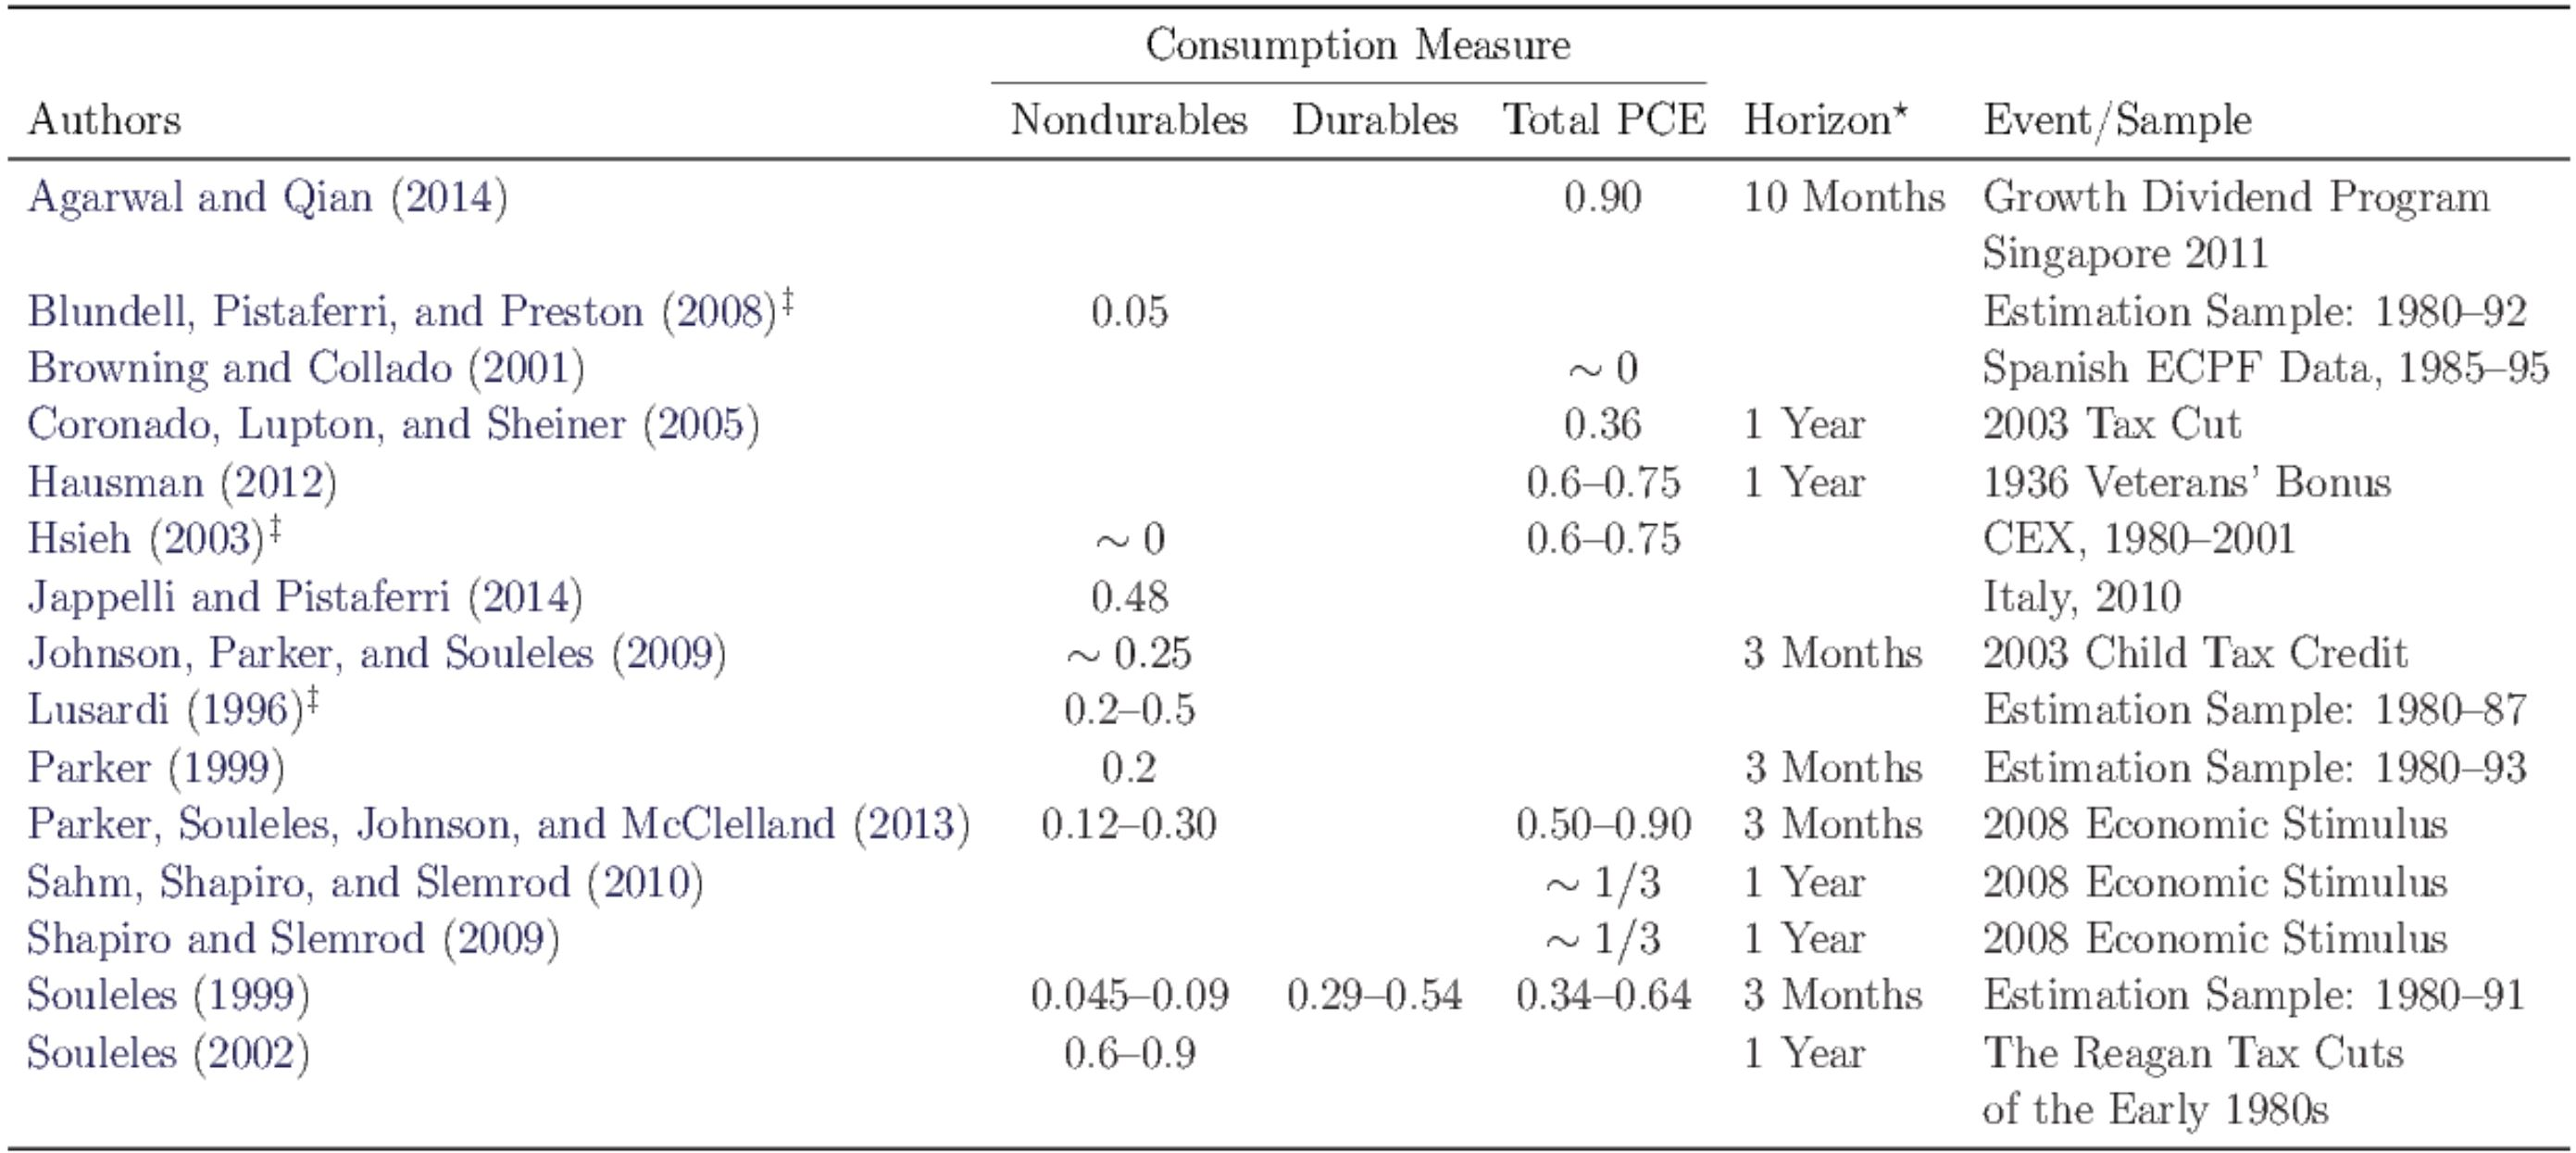
\includegraphics[height=5cm]{../Figures/MPCEmpiricalTable}};
	\pause
	\node (img2) at (img1) 		{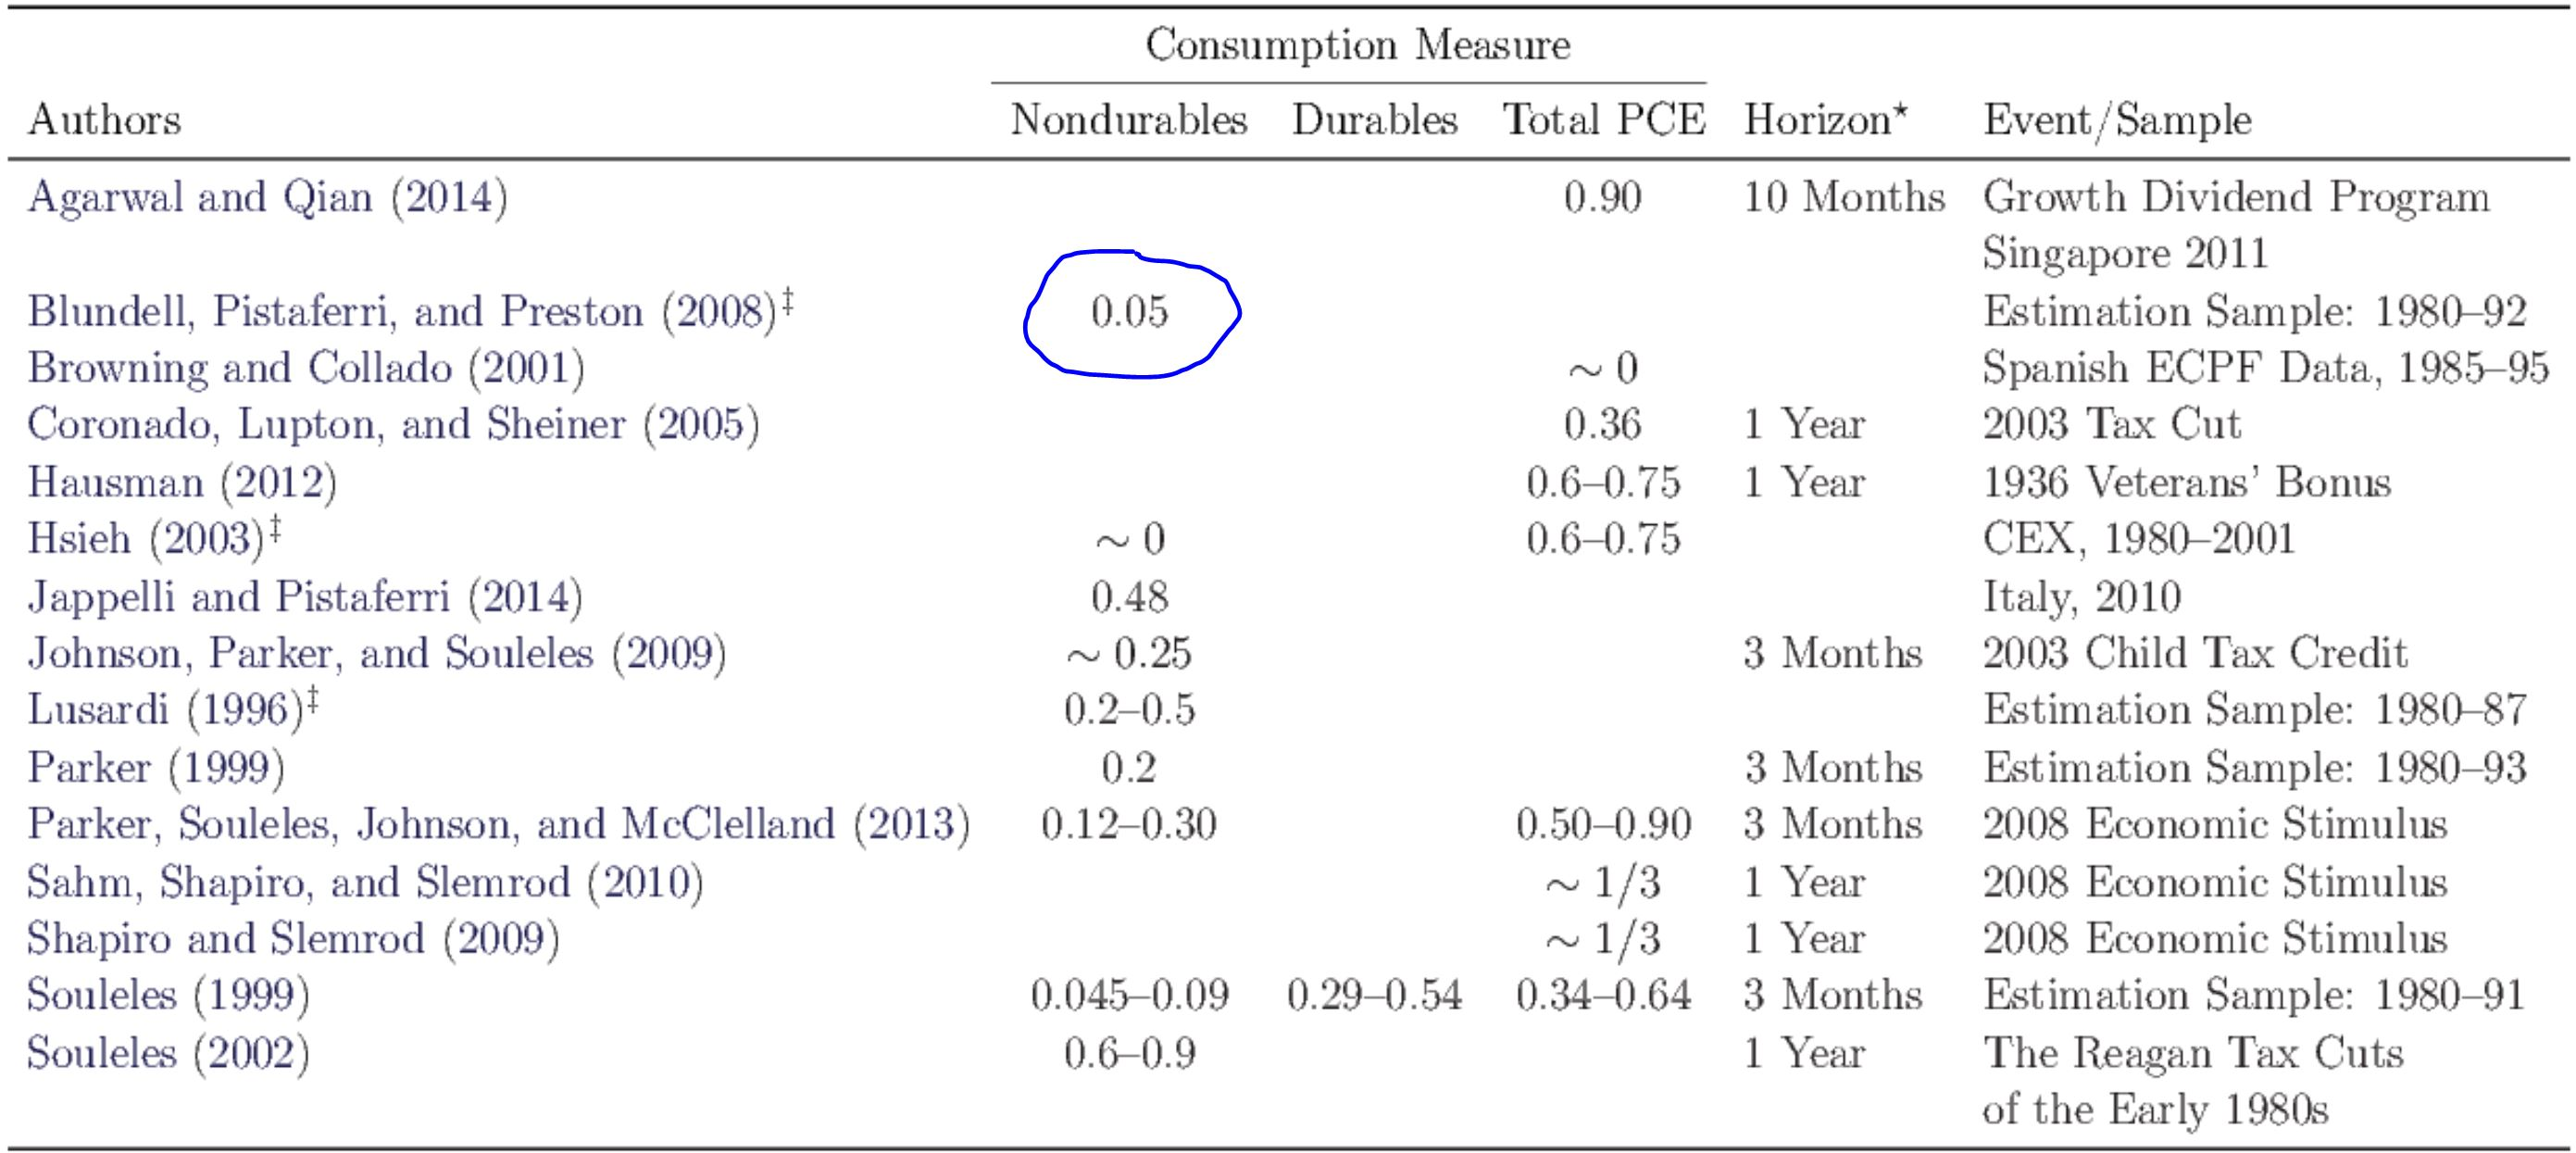
\includegraphics[height=5cm]{../Figures/MPCEmpiricalTable2}};
	\end{tikzpicture}
	\tiny{Table from Carroll et al 2018}
\end{center}
Rough consensus on (3 month) MPC $\sim 30\%$
}
\frame
{
	\frametitle{Empirical Evidence on the Distribution of MPC}
	Auclert (2018) uses the 3 different methods to identify the distribution of MPC by unhedged interest rate exposure
	\begin{figure}
		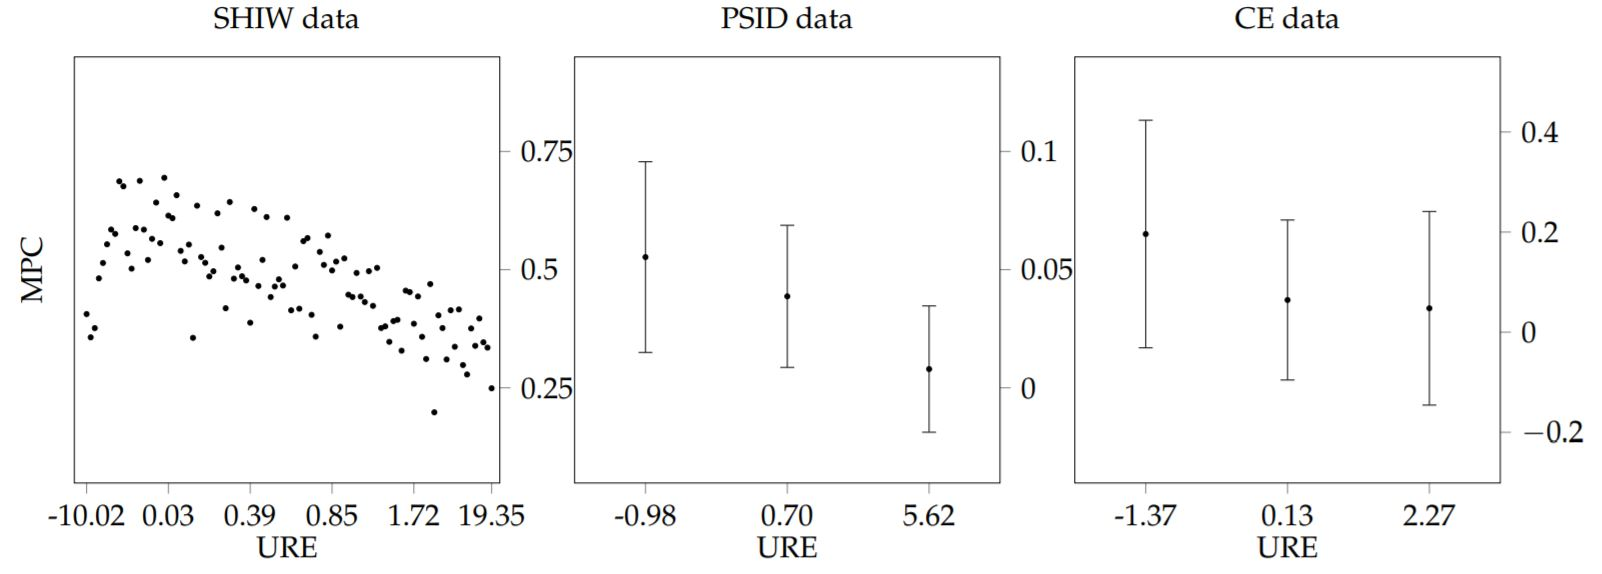
\includegraphics[scale=0.6]{../Figures/MPCDistributionAuclert}
	\end{figure}
	Recent evidence from Norwegian registry data using lottery winnings provides evidence of variation across liquid wealth
}
\frame{
	\frametitle{Results Preview}
	Spending is VERY closely tied with transitory income\\
	\begin{itemize}
		\item Far more than standard models would suggest
	\end{itemize}
	High levels of liquid wealth reduce this relation
	\begin{itemize}
		\item As standard models suggest
	\end{itemize}
	\pause
	\bigskip
	\$1000 of extra transitory income in a year is associated with \$700 of extra spending that year\\
	\bigskip
	Possible Interpretation:
	\begin{itemize}
		\item Labor supply responds to transitory spending needs
		\item eg Car break down, work extra hours
	\end{itemize}
}
\begin{comment}
\frame
{
	\frametitle{Range of Theories}
	\begin{itemize}
		\item Complete Markets: No consumption response to idiosyncratic income shocks
		\item Permanent Income Hypothesis: MPC out of permanent income is 1, out of transitory is 0
		\item Standard incomplete market model: Somewhere in between. Depends strongly on wealth and income uncertainty
		\item Two asset models: Depends strongly on liquid wealth
	\end{itemize}

}
\end{comment}
\section{Empirical Strategy}
\setbeamercovered{invisible}
\frame
{
	\frametitle{Blundell Pistaferri and Preston 2008}
	Question:\\
	\bigskip
	\qquad \textit{How well insured are households against idiosyncratic income shocks?}\\
	\bigskip
	Key idea: 
	\begin{itemize}
		\item[1] Make a few core assumptions on the dynamics of income and consumption
		\item[2] Use the covariance matrix of income and consumption to identify key parameters
		\begin{itemize}
			\item $\phi \approx 0.65$ Partial permanent shock insurance
			\item $\psi \approx 0.05$ Almost complete transitory shock insurance
		\end{itemize}
	\end{itemize}
	\pause
	Kaplan \& Violante (2010)``The BPP insurance coefficients should become central in quantitative macroeconomics"
}
\frame
{
	\frametitle{Blundell Pistaferri and Preston 2008}
	Assumptions on the log income process
	\begin{itemize}
		\item $y_t = p_t + \varepsilon_t$
		\item $p_t = p_{t-1} + \zeta_t$
	\end{itemize}
	Standard Friedman transitory/permanent decomposition (can easily extend to an MA(q) transitory process)\\
	\pause
	\bigskip
	Assumptions on the log consumption process
	\begin{itemize}
		\item $\Delta c_t = \phi \Delta p_t + \psi \varepsilon_t$
	\end{itemize}
	Hall random walk\\
}
\frame
{
	\frametitle{BPP: Identification}
	Key identification moments for $\phi$ and $\psi$
	\begin{align*}
		\phi &= \frac{\mathrm{Cov}(\Delta c_t, \zeta_t)}{\mathrm{Var}(\zeta_t)}\\
		     &= \frac{\mathrm{Cov}(\Delta c_t, \Delta y_{t+1}+ \Delta y_t+ \Delta y_{t-1}))}{\mathrm{Cov}(\Delta y_t, \Delta y_{t+1}+ \Delta y_t+ \Delta y_{t-1})}\\
		\\
		\psi &= \frac{\mathrm{Cov}(\Delta c_t, \varepsilon_t)}{\mathrm{Var}(\varepsilon_t)}\\
		&= \frac{\mathrm{Cov}(\Delta c_t, \Delta y_{t+1})}{\mathrm{Cov}( \Delta y_t, \Delta y_{t+1})}
	\end{align*}
		Kaplan \& Violante (2010) show these work well for reasonable parameterizations of standard consumption models
}
\frame
{
	\frametitle{BPP: Two Improvements}
	\begin{itemize}
		\item Time Aggregation
		\item Short term dynamics
	\end{itemize}
}
\frame
{
	\frametitle{BPP: Time Aggregation}
	Working (1960) showed that the a time aggregated random walk is autocorrelated
	\begin{figure}
		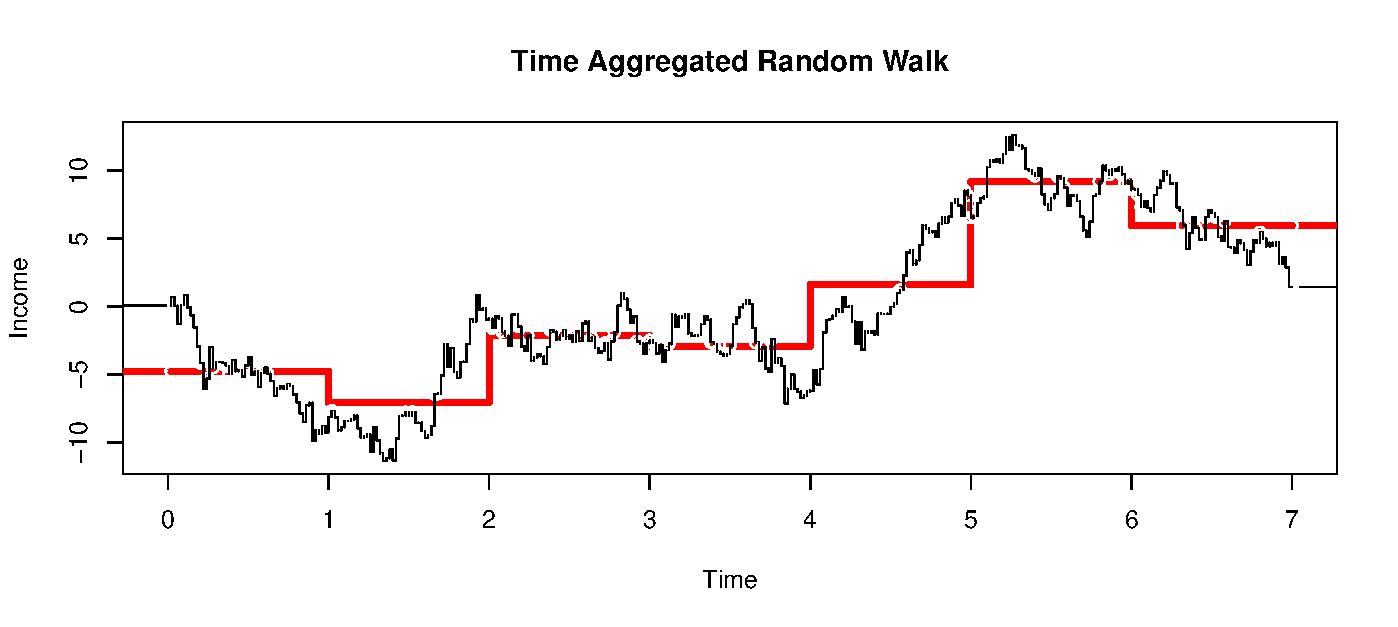
\includegraphics[scale=0.4]{../Figures/timeagg_rw.pdf}
	\end{figure}
	\pause
	Macroeconomics has (mostly) absorbed this point\\
	The household finance literature has not - this is particularly problematic for BPP
}
\frame
{
	\frametitle{BPP: Time Aggregation}
	BPP use the (non time-aggregated) moment
	\begin{align*}
		\frac{\mathrm{Cov}(\Delta c_t, \Delta y_{t+1})}{\mathrm{Cov}( \Delta y_t, \Delta y_{t+1})} &= \frac{-\psi \mathrm{Var}(\varepsilon)}{-\mathrm{Var}( \varepsilon)}= \psi
	\end{align*}
	\pause
	But if the underlying processes are continuous
	\begin{align*}
	\frac{\mathrm{Cov}(\Delta \bar{c_t}, \Delta \bar{y}_{t+1})}{\mathrm{Cov}( \Delta \bar{y}_t, \Delta \bar{y}_{t+1})}
	&= \frac{ \frac{1}{6}\phi \mathrm{Var}(\zeta) - \frac{1}{2}\psi \mathrm{Var}(\varepsilon)}{ \frac{1}{6} \mathrm{Var}(\zeta) -  \mathrm{Var}(\varepsilon)}
	\end{align*}
	So the moment used for identification of $\psi$ is messed up
}
\frame
{
	\frametitle{BPP Time Aggregation Problem}
	Problem: BPP estimates (from PSID data) are wildly out of sync with the rest of the literature\\
	\bigskip
	MPC out of transitory estimate:  $\sim 5\%$\\
	MPC out of permanent estimate:  $\sim 65\%$ \\
	\pause
	\bigskip
	Fixing time aggregation we get\\
	\bigskip
	MPC out of transitory estimate:  $\sim 25\%$\\
	MPC out of permanent estimate:  $\sim 30-100\%$ \\
	\bigskip
	Results become VERY sensitive to exact nature of short term income dynamics
}
\frame
{
	\frametitle{BPP Short Term Dynamics}
	Identification in BPP comes primarily from covariances from one period to the next\\
	\bigskip
	Carroll \& Samwick (1997) use a similar technique to identify shock variances, but use a longer time frame
	\begin{align*}
		\mathrm{Var}(\Delta^n y_t) = n \mathrm{Var} (\zeta) + 2 \mathrm{Var}(\varepsilon)
	\end{align*}
	Using $n=3,4,5$ the identification is robust to MA(2) transitory shocks\\
	\bigskip
	\pause
	\begin{itemize}
		\item[1] What might the equivalent of ``robust to MA(2) transitory shocks" be in continuous time?
		\item[2] Can we extend this more robust method to consumption?
	\end{itemize}
}
\frame
{
	\frametitle{BPP Short Term Dynamics}
	Carroll \& Samwick in Discrete Time
	\begin{figure}
	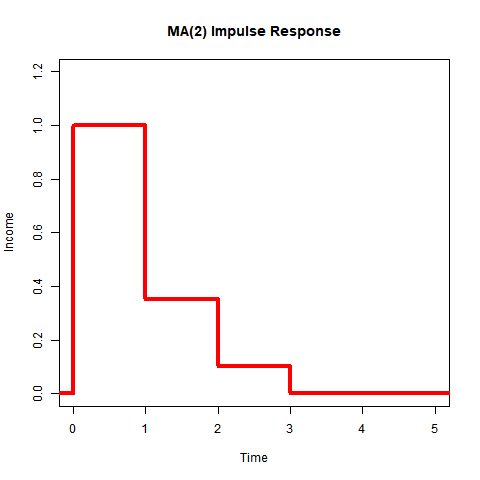
\includegraphics[scale=0.3]{../Figures/MA2.png}
	\end{figure}
	\begin{align*}
		y_t &= p_t + \varepsilon_t + \theta_1 \varepsilon_{t-1} + \theta_2 \varepsilon_{t-2} \\
		p_t &= p_{t-1} +\zeta_t\\
		\implies \mathrm{Var}(\Delta^n y_t) &= n \mathrm{Var}(\zeta) + 2\underbrace{(1+\theta_1^2 + \theta_2^2)\mathrm{Var}(\varepsilon)}_\text{``Total" transitory variance} \qquad \text{ for $n \geq 3$} \\
	\end{align*}	

}
\frame
{
	\frametitle{BPP Short Term Dynamics}
	Carroll \& Samwick in Continuous Time with Aggregation\\
	\bigskip
	To begin assume no persistence in the transitory shock
	\begin{align*}
		y_t dt = p_t dt + dq_t
	\end{align*}
	where $p_t$ and $q_t$ are independent stationary martingale processes with variances $\sigma^2_p$ and $\sigma^2_q$
	\begin{align*}
	\bar{y}_T &= \int_{T-1}^{T}p_t dt + \int_{T-1}^{T}dq_t \\
	\implies  \mathrm{Var}(\Delta^n \bar{y}_T) &= (n-\frac{1}{3})\sigma_p + 2\sigma_q
	\end{align*}
}
\frame
{
	\frametitle{BPP Short Term Dynamics}
	Allow a generic transitory shock, $f(t)$ where $f(t)=0$ if $t>2$
	\begin{figure}
		\includegraphics[scale=0.3]{../Figures/GenericTransitory.png}
	\end{figure}
	\vspace*{-0.3in}
	\begin{align*}
	y_t &= p_t + \int_{t-2}^{t} f(s-(t-2))dq_s\\
	\implies \mathrm{Var}(\Delta^n \bar{y}_T) &= (n-\frac{1}{3})\sigma^2_p +  2 \mathrm{Var}(\tilde{y}) \text{   for }n \geq 3
	\end{align*}	
	where $	\tilde{y_T} = \int_{T-1}^{T}\int_{t-2}^{t} f(s-(t-2))dq_s dt$ is the time aggregated transitory component of income
}
\frame
{
	\frametitle{BPP Short Term Dynamics}
	Assumptions on Consumption\\
	\begin{itemize}
		\item Permanent: Same as BPP $c_t = \phi y_t$ (+constant)
		\item Transitory: Allow for generic impulse response $g(t)$ where $g(t) = 0$ for $t>2$
	\end{itemize}
	\vspace*{-0.2in}
	\begin{center}
	\begin{tikzpicture}
	\node (img1) {\includegraphics[height=4cm]{../Figures/GenericTransitoryConsumption.png}};
	\pause
	\node (img2) at (img1) {\includegraphics[height=4cm]{../Figures/GenericTransitoryConsumptionWithBPP.png}};
	\end{tikzpicture}
	\end{center}
	\vspace*{-0.2in}
	This is a key difference between what we assume and BPP
}
\frame
{
	\frametitle{BPP Short Term Dynamics}
	\begin{align*}
	c_t dt &= \phi y_t dt + \int_{t-2}^{t} g(s-(t-2))dq_s dt \\
	\implies \mathrm{Cov}(\Delta^n \bar{c_T},\Delta^n \bar{y_T} ) &= \phi (n-\frac{1}{3}) \sigma^2_p + 2 \mathrm{Cov}(\tilde{c},\tilde{y})
	\end{align*}
	where $\tilde{c}$ and $\tilde{y}$ are the time aggregated \textit{transitory} components of consumption and income	\\
}
\frame
{
	\frametitle{BPP Short Term Dynamics}
	Is 2 years long enough?
    \begin{columns}
	\column{0.5\linewidth}
	\centering
	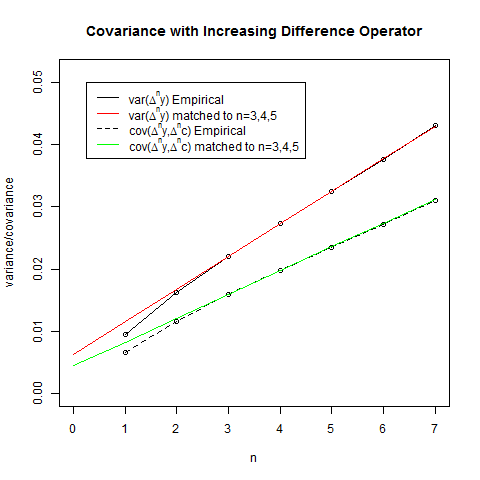
\includegraphics[scale=0.35]{../Figures/IncreasingDiff.png}
	\column{0.5\linewidth}
	Should be linear in $n$:
	\begin{align*}
		\mathrm{Var}(\Delta^n \bar{y}_T) = (n-\frac{1}{3})\sigma_p + 2\mathrm{Var}(\tilde{y}) \\[5pt]
		\mathrm{Cov}(\Delta^n \bar{y}_T, \Delta^n \bar{c}_T) \qquad \qquad \qquad \\
		\qquad = \phi(n-\frac{1}{3})\sigma_p + 2\mathrm{Cov}(\tilde{c},\tilde{y})
	\end{align*}
	\end{columns} 
}
\frame
{
	\frametitle{BPP Short Term Dynamics}
	We can now identify:
	\begin{itemize}
		\item $\sigma^2_p$ Variance of permanent shocks
		\item $\mathrm{Var}(\tilde{y})$ Variance of transitory income received in a year
		\item $\phi$ Elasticity of consumption w.r.t permanent income
		\item $\psi = \frac{\mathrm{Cov}(\tilde{c},\tilde{y})}{\mathrm{Var}(\tilde{y})}$ Elasticity of transitory consumption w.r.t transitory income over a year
	\end{itemize}
	\pause
	$\psi=0.7$ means \textit{``If income this year is 1\% higher than it would have been with no transitory shocks this year or in the last 2 years, then consumption is on average 0.7\% higher than it would have been''}\\
	\bigskip
	or equivalently $\psi$ is \textit{the regression coefficient of transitory consumption on transitory income over a one year period}
}
\section{Data}
\frame
{
	\frametitle{Data}
	\begin{itemize}
		\item Starting point: Register based micro data for all Danish households made available by Statistics Denmark
		\item Really good income data
		\begin{itemize}
			\item We use total income (i.e. labor income, transfers, and capital income) after tax, based on third-party reported tax data
		\end{itemize}
		\item Work with the residual of log income after controlling for age, education, marital status etc. (along with interactions of these)
		\item Expenditure data imputed from income and wealth
		\begin{itemize}
			\item Deposit and brokerage accounts all third party reported
			\item Less accurate than income data
		\end{itemize}
	\end{itemize}
}
\frame
{
	\frametitle{Imputing Expenditure}
	We use the identity
		\begin{align*}
			C_t \equiv Y_t - S_t = Y_t - \Delta NW
		\end{align*}
	\begin{itemize}
		\item Works well for households with simple financial lives
		\item Main issue: Capital gains and losses
		\begin{itemize}
			\item Exclude households where methodology will not work well (eg Business owners)
			\item Exclude housing wealth and years with housing transactions
			\item Capital gains for stocks based on a diversified index
		\end{itemize}
		\item Noisy, but perhaps better than surveys (Browning and Leth-Petersen, 2003; Eika et al., 2017; Fagereng and Halvorsen, 2017; Koijen et al., 2015; Kolsrod et al., 2017; Kreiner et al., 2015)
		\item Huge sample size advantage: sample covers 23.3 million observations over 2004-2015 (approx 1.9 million per year)
	\end{itemize}
}
\section{Results}
\frame
{
	\frametitle{Results Overview}
	\begin{itemize}
		\item Elasticity of consumption with transitory income is VERY high
		\item Lots of heterogeneity in transitory and permanent variance
		\item Surprisingly little heterogeneity in either transitory or permanent consumption responses
		\item Low liquid wealth associated with high $\phi$ and $\psi$
	\end{itemize}
	\pause
	Possible explanations
	\begin{itemize}
	\item MPC is much higher than we think
	\item Income variance reflects choices, not exogenous risk 
	\item Measurement error
	\end{itemize}
}
\frame
{
	\frametitle{Shock Variance by Age}
	\begin{figure}
		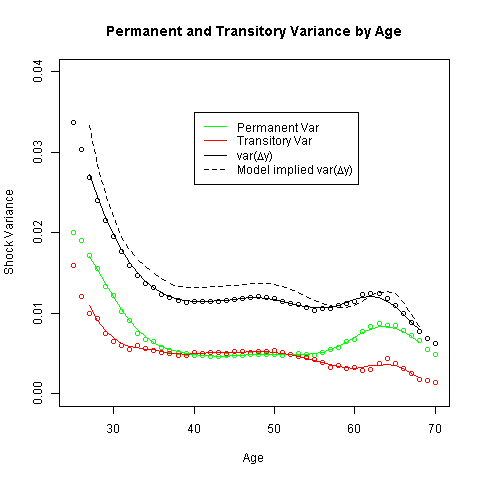
\includegraphics[scale=0.35]{../Figures/VarianceByAge.png}
	\end{figure}
	\vspace{-0.25in}
	The assumption of constant variance works well from mid-30's to retirement
}
\frame
{
	\frametitle{MPX by Age}
	\begin{columns}
		\column{0.5\linewidth}
		\centering
		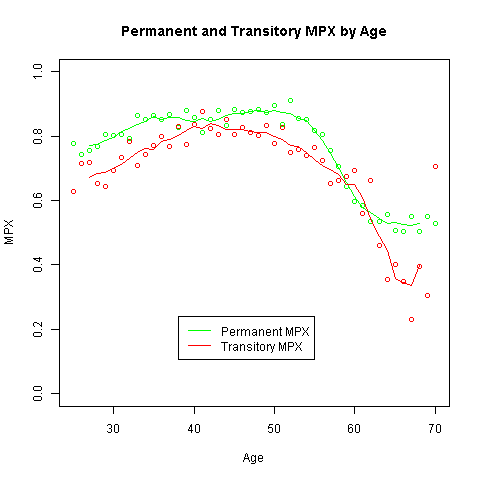
\includegraphics[scale=0.35]{../Figures/MPXByAge.png}
		\column{0.5\linewidth}
		\begin{itemize}
			\item MPX is very high
			\item No large difference between permanent and transitory MPX
			\item Both decline towards retirement
		\end{itemize}
	\end{columns} 	
}
\frame
{
	\frametitle{MPX by Liquid Wealth}
	\begin{columns}
		\column{0.5\linewidth}
		\centering
		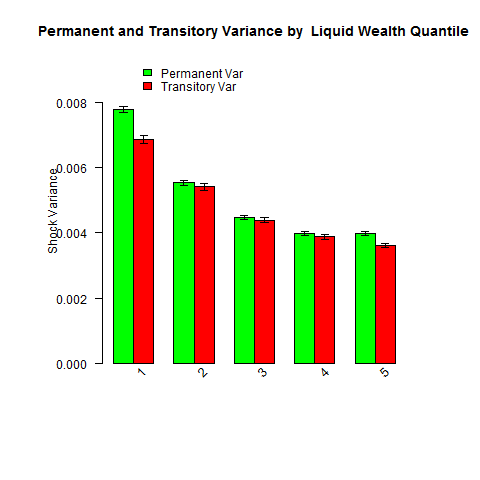
\includegraphics[scale=0.35]{../Figures/VarianceByLiquidWealth.png}
		\column{0.5\linewidth}
		\centering
		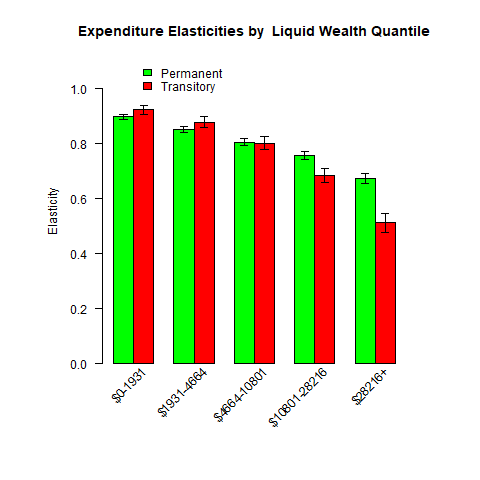
\includegraphics[scale=0.35]{../Figures/MPXByLiquidWealth.png}
	\end{columns} 	
}
\frame
{
	\frametitle{Little Relation between Shock Variance and MPX}
	\begin{columns}
		\column{0.5\linewidth}
		\centering
		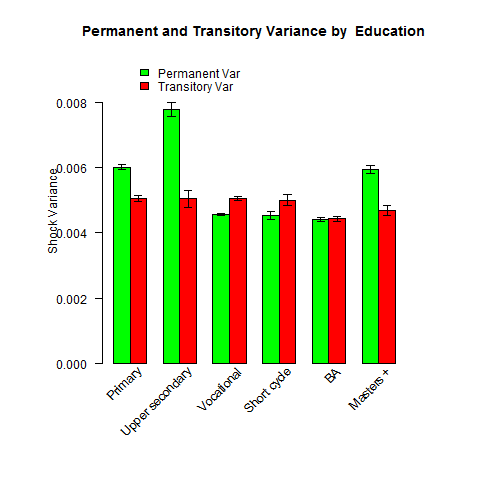
\includegraphics[scale=0.2]{../Figures/VarianceByEducation.png}\\
		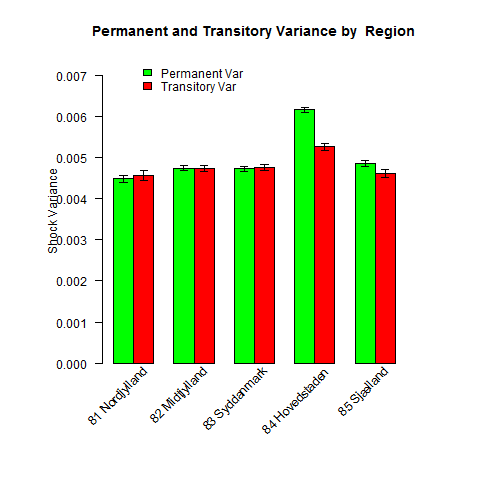
\includegraphics[scale=0.2]{../Figures/VarianceByRegion.png}
		\column{0.5\linewidth}
		\centering
		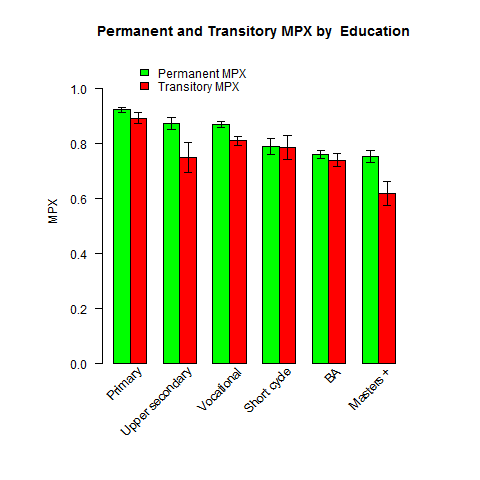
\includegraphics[scale=0.2]{../Figures/MPXByEducation.png}\\
		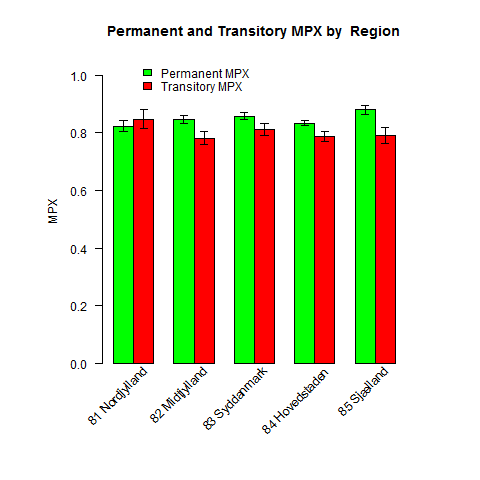
\includegraphics[scale=0.2]{../Figures/MPXByRegion.png}
	\end{columns} 
}
\frame
{
	\frametitle{Sensitivity to Misspecification}
	Given the MPX out of transitory and permanent income are both similar, results are not very sensitive to exact modeling assumptions
	\begin{itemize}
		\item AR(1) in permanent shock
		\item Correlation between permanent and transitory shocks
	\end{itemize}
}
\frame
{
	\frametitle{Why is Transitory MPX so large?}
	Explantion 1: It just is \\
	\bigskip
	In line with some other estimates e.g.
	\begin{itemize}
		\item Agarwal \& Quin (2014) find 90\% 10 month MPX from the 2011 Singapore Growth Dividend Program (excellent data)
		\item Parker et al. (2013) find 50-90\% 3 month MPX out of 2008 stimulus
		\item Souleles (2002) finds 60-90\% 12 month MPX out of Reagan tax cuts
	\end{itemize}
	\pause
	However, Fagereng et al (2017) find an MPX of 35\% using lottery winnings and similar expenditure data in Norway

}
\frame
{
	\frametitle{Why is Transitory MPX so large?}
	Explantion 2: Income is Endogenous\\
	\bigskip
	Potential model would need
	\begin{itemize}
		\item Permanent and transitory income uncertainty
		\item Transitory taste shocks
		\item Endogenous labor supply
	\end{itemize}
	Is a quantitatively reasonable model feasible?
	\begin{itemize}
	\item How big (or small) will labor elasticity need to be?
	\item Seems unlikely the high wealthy MPX can be matched
\end{itemize}
}
\frame
{
	\frametitle{Why is Transitory MPX so large?}
	Explantion 3: Measurement Error\\
	\bigskip
	\begin{itemize}
		\item Method is robust to \textit{classical} measurement error in expenditure
		\item Method is (mostly) robust to \textit{classical} measurement error in income
		\item The imputation method potentially introduces correlation between measurement error in income and expenditure (a problem)
	\end{itemize}
	Unobserved income uncorrelated with observed income is OK\\
	Problem if income is observed with error
}
\section{Way Forward}
\frame
{
	\frametitle{Why is Transitory MPX so large?}
	How can we dig into this?\\
	\bigskip
	\begin{itemize}
		\item Break down sources of income
		\begin{itemize}
			\item MPX from secondary earner is much higher than primary earner
			\item Look only at households who have little choice over work hours
			\item Look at wages and hours worked rather than income
		\end{itemize}	
		\item Use income data from an independent source (employer payment data)
	\end{itemize}
}
\frame
{
	\frametitle{Model}
	How will a model in which labor decisions are driven by spending needs behave over the business cycle?\\
	\begin{itemize}
		\item In a recession households have much less ability to insure themselves through their labor supply
		\item May increase saving to compensate
	\end{itemize}
}
\frame
{
	\frametitle{Model}
	GHH preferences with a taste shifter
	\begin{align*}
	u(c,l,\varphi) &= U(\varphi c - G(l))
	\end{align*}
	First order condition w.r.t $l$
	\begin{align*}
	\implies l = G^{'-1}(\varphi w)
	\end{align*}
	where $w$ is the wage\\
	\bigskip
	Note - even the wealthy adjust their labor
}
\end{document}


